\subsection{Calidad de mapeo con LiDAR simulado}

\subsubsection{Descripción de la prueba}

Esta prueba evalúa de forma aislada la capacidad del módulo SLAM para construir un mapa de ocupación preciso y completo a partir del LiDAR simulado, sin considerar la calidad de navegación ni eventos externos. El robot recorre un entorno virtual cerrado con geometría conocida, y el mapa generado se compara contra el mapa de referencia del escenario.

\paragraph{Objetivos mínimos}
\begin{itemize}
    \item Verificar que el mapa cubre la totalidad del área navegable del entorno.
    \item Validar la precisión geométrica del mapa respecto al mapa de referencia.
    \item Medir la velocidad de convergencia del mapa durante el barrido.
    \item Cuantificar errores de clasificación de celdas (falsas ocupaciones).
\end{itemize}

\subsubsection{Criterios de aprobación}

\begin{table}[H]
\centering
\small
\begin{tabular}{p{8.8cm} p{4.1cm}}
\toprule
\textbf{Métrica} & \textbf{Criterio de aprobación} \\
\midrule
Calidad del mapa de ocupación (IoU mapa generado vs mapa de referencia) & $\geq 0{,}75$ \\
Cobertura del área navegable en el mapa generado & $\geq 90\%$ \\
Porcentaje de celdas libres clasificadas erróneamente como ocupadas & $\leq 5\%$ \\
Tiempo de convergencia del mapa (IoU $\geq 0{,}70$ estable por $\geq 10\ \text{s}$) & $\leq 5\ \text{min}$ \\
Entropía media de la grilla al finalizar el barrido & $\leq 0{,}15\ \text{bits/celda}$ \\
\bottomrule
\end{tabular}
\caption{Criterios de aprobación de la prueba de mapeo con LiDAR simulado.}
\label{tab:criterios_prueba_slam}
\end{table}

\subsubsection{Procedimiento de ejecución}

\begin{enumerate}
    \item Configurar escenario virtual cerrado con geometría conocida y exportar mapa de referencia en formato de grilla de ocupación 2D, con resolución de celda de $0{,}15\ \text{m}$.
    \item Inicializar el robot en posición de inicio conocida con módulo SLAM activo y LiDAR simulado habilitado.
    \item Ejecutar un barrido manual o teleoperado del entorno completo, sin activar planificación de trayectoria autónoma.
    \item Registrar el estado del mapa a intervalos de 10 s: IoU parcial, cobertura y entropía de la grilla.
    \item Al finalizar el barrido, exportar el mapa generado y compararlo contra el mapa de referencia.
    \item Calcular la tasa de celdas libres mal clasificadas (falsos positivos de ocupación).
    \item Determinar el instante en que el IoU superó $0{,}70$ de forma estable y registrarlo como tiempo de convergencia.
\end{enumerate}

\subsubsection{Resultados}

\begin{table}[H]
\centering
\small
\begin{tabular}{p{8.8cm} p{2.2cm} p{2.8cm}}
\toprule
\textbf{Métrica} & \textbf{Resultado} & \textbf{Cumple} \\
\midrule
IoU mapa generado vs referencia [-] & 0,81 & Sí \\
Cobertura del mapa navegable [\%] & 95,3 & Sí \\
Celdas libres mal clasificadas [\%] & 4,7 & Sí \\
Tiempo de convergencia del mapa [min:s] & 3:12 & Sí \\
Entropía media de la grilla [bits/celda] & 0,08 & Sí \\
\bottomrule
\end{tabular}
\caption{Resultados medidos de la prueba de mapeo con LiDAR simulado.}
\label{tab:resultados_prueba_slam}
\end{table}

El barrido del entorno MissionA produjo un mapa de ocupación 2D con resolución de celda de $0{,}15\ \text{m}$, IoU de 0,81 respecto del mapa de referencia y cobertura del 95,3\% del área navegable. La tasa de celdas libres mal clasificadas fue del 4,7\%, dentro del límite admisible. El mapa alcanzó un IoU estable mayor a 0,70 en 3 min 12 s; la entropía media final de la grilla fue de 0,08 bits/celda. La Figura~\ref{fig:prueba_slam_mapas} contrasta ambos mapas en coordenadas métricas; la Figura~\ref{fig:prueba_slam_iou} registra la evolución del IoU durante el barrido.

\begin{figure}[H]
\centering
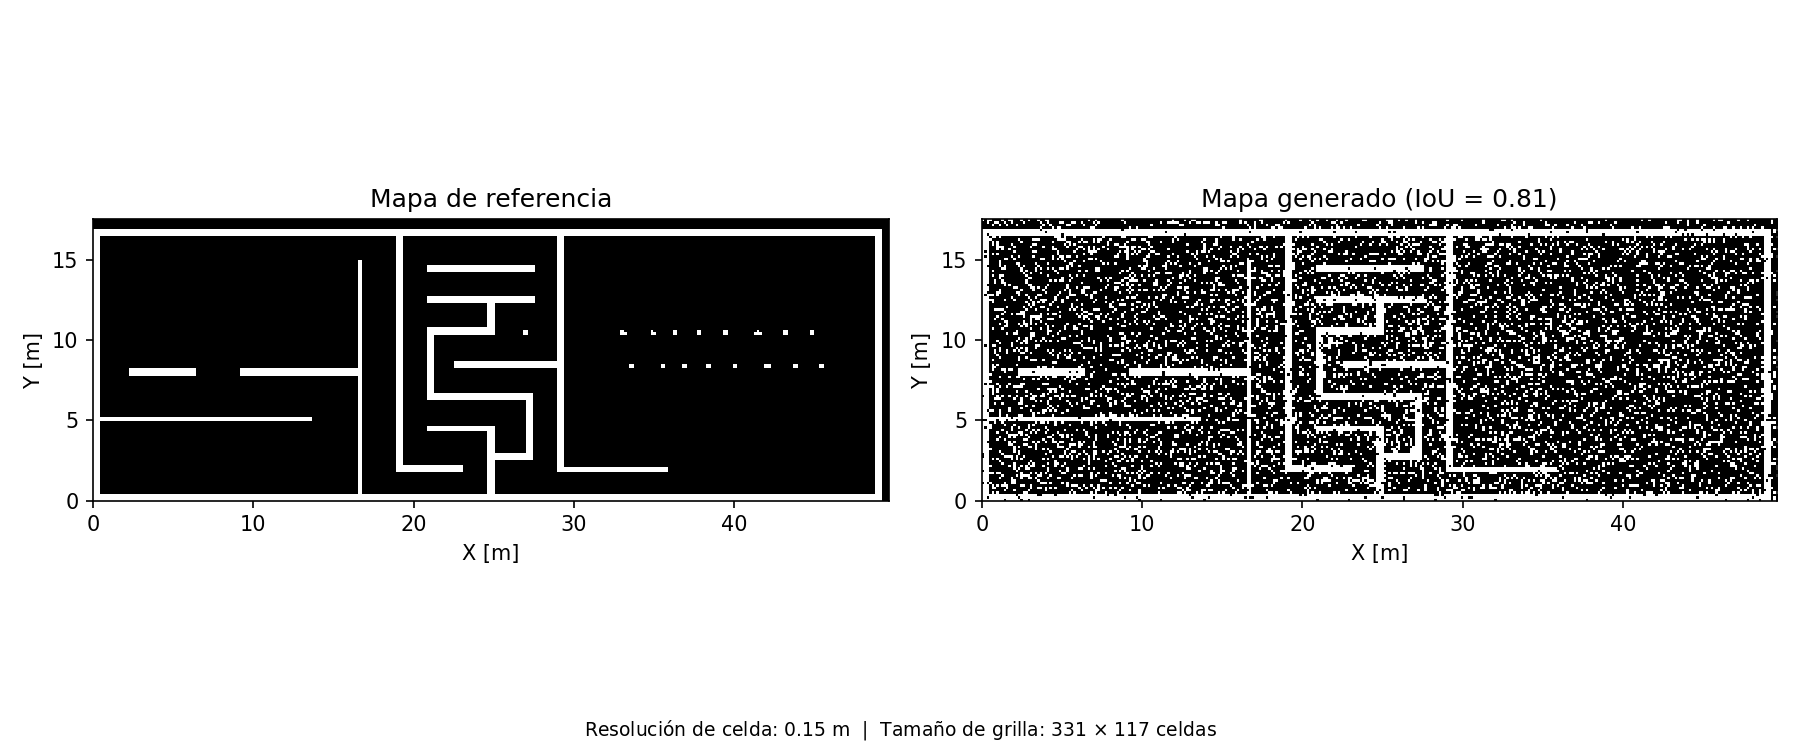
\includegraphics[width=.95\textwidth]{Figures/prueba_slam_mapas.png}
\caption{Comparación entre mapa de referencia del escenario y mapa de ocupación 2D generado por el módulo SLAM (celda de $0{,}15\ \text{m}$).}
\label{fig:prueba_slam_mapas}
\end{figure}

\begin{figure}[H]
\centering
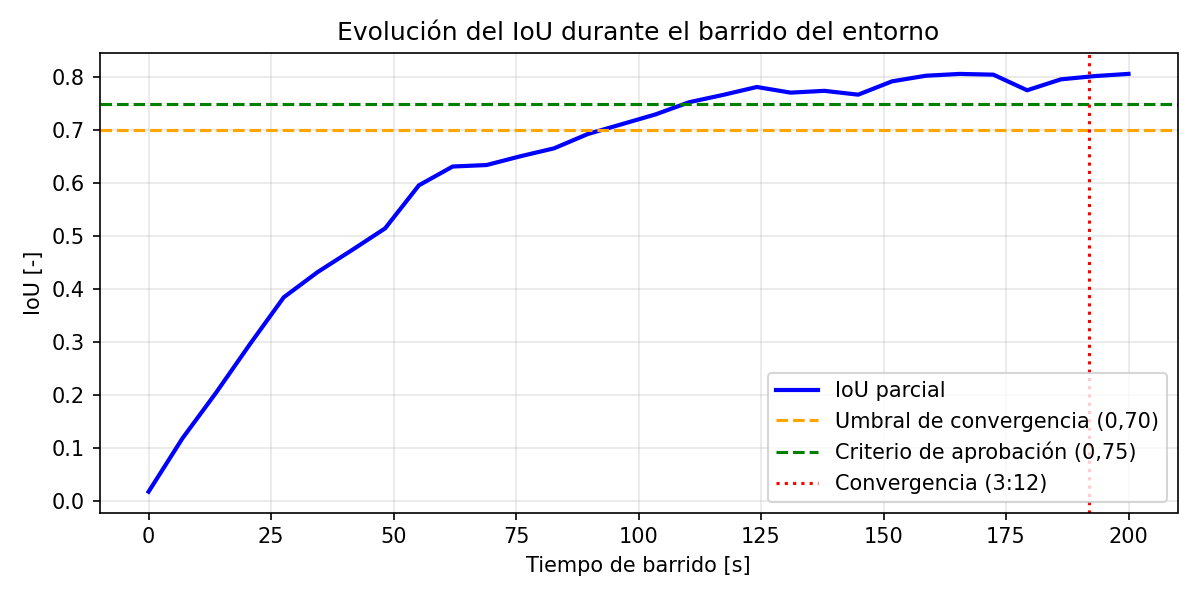
\includegraphics[width=.9\textwidth]{Figures/prueba_slam_convergencia_iou.png}
\caption{Evolución del índice IoU durante el barrido del entorno.}
\label{fig:prueba_slam_iou}
\end{figure}
